%!TEX root = report.tex
To test if the ratio of autonomous vehicles to human driven vehicles influences the flow of traffic and the number of collisions we run our simulation in batch mode with different initialisations. \Cref{ss:method:experiment:init} presents the different initialisations we used, \cref{ss:method:experiment:measures} discusses what measure, how we measure it en how it relates to real world traffic. 

\subsubsection{Initialisation}
\label{ss:method:experiment:init}
As described in \cref{ss:method:experiment:init} we need to decide on a graph to use and the ratio of human driven vehicles to autonomous cars. 

We measure the influence of adding self-driving cars to traffic in two different graphs, both are presented in c


\begin{figure}
	\centering
	\begin{subfigure}{0.45\textwidth}
		\centering
		% 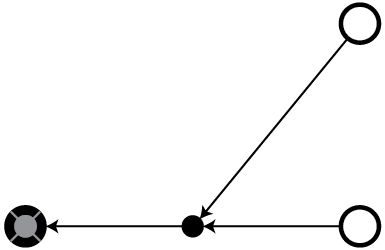
\includegraphics[width=\textwidth]{./img/method_experiment_merging}
	\begin{tikzpicture}[shorten >=1pt,node distance=2cm,auto]

		\node[state,initial, initial text={}]   (q_0)                 		{$q_0$};
		\node[state, accepting]           		(q_1) [above of=q_0]        {$q_1$};
		\node[state, accepting]           		(q_2) [below of=q_0]        {$q_2$};
		\node[state, accepting]           		(q_3) [right of=q_0]        {$q_3$};

		\path[->]		(q_0) edge	[loop left]			node		{$a \; \varepsilon/A$}							();
		\path[->]		(q_0) edge						node		{$b \; \varepsilon/\varepsilon$}				(q_1);
		\path[->]		(q_0) edge						node		{$\varepsilon \; \varepsilon/\varepsilon$}		(q_2);
		\path[->]		(q_0) edge						node		{$\varepsilon \; \varepsilon/\varepsilon$}		(q_3);
		\path[->]		(q_1) edge	[loop right]		node		{$a \; A/\varepsilon$}							();
		\path[->]		(q_2) edge	[loop right]		node		{$a \; \varepsilon/\varepsilon$}				();
		\path[->]		(q_3) edge	[loop right]		node		{$b \; \varepsilon/\varepsilon$}				();
	\end{tikzpicture}		
		\caption{Merging traffic}
		\label{fig:method:experiment:merging}
	\end{subfigure}
	\begin{subfigure}{0.45\textwidth}
		\centering
		% 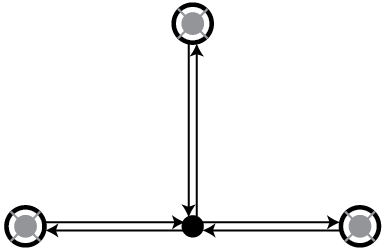
\includegraphics[width=\textwidth]{./img/method_experiment_intersection}
		\missingfigure{Intersection}
		\caption{Intersecting traffic}
		\label{fig:method:experiment:intersection}
	\end{subfigure}	
	\caption{The graphs representing the network of streets used in our experiment, \subref{fig:method:experiment:merging} shows a graph that forces traffic to merge into a different lane with traffic, \subref{fig:method:experiment:intersection} presents a graph that forces cars to cross other traffic.}
	\label{fig:method:experiment}
\end{figure}
% Welke grafen gebruiken we
% Welke ratios gebruiken we

\subsubsection{Measures}
\label{ss:method:experiment:measures}
% Wat meten we, hoe heeft dat relatie met RL
% Hoe meten we het





% To test if autonomous vehicles have an influence on traffic delays and crashes, we run the simulation multiple times, with different autonomous vehicle to human driver ratios.

% For each of these runs, we measure the time it takes for each agent to reach its goal, relative to the distance they have to travel from their initial position to the target. Furthermore we keep track of the number of collisions with other agents. 

% Using these measurements, we  determine if the number of collisions and the delay time are influenced by the ratio of autonomous agents to the human ones. 

% \baakman{Welke statistieken hebben we? Hoe rekenen we ze uit? Waarom zijn ze relevant.}

% \baakman{Welke twee grafen (Invoegen, T-splitsing) gebruiken we, waarom deze, plaatjes enzo.}

% \baakman{Hoe vaak runnen we, met welke initiele parameters runnen we. Hoe lang runnen we.}